\documentclass{beamer}
\usetheme{Singapore}
\usepackage{changepage}

%\usepackage{pstricks,pst-node,pst-tree}
\usepackage{amssymb,latexsym}
\usepackage{tikz}
\usepackage{graphicx}
\usepackage{fancyvrb}
\usepackage{hyperref}
\usepackage{fancybox}
\usepackage[listings]{tcolorbox}

\definecolor{codegreen}{rgb}{0,0.6,0}
\definecolor{codegray}{rgb}{0.5,0.5,0.5}
\definecolor{codepurple}{rgb}{0.58,0,0.82}
\definecolor{backcolour}{rgb}{0.95,0.95,0.92}

\lstdefinestyle{mystyle}{
    language=Python,
    backgroundcolor=\color{backcolour},   
    commentstyle=\color{codegreen},
    keywordstyle=\color{magenta},
    numberstyle=\tiny\color{codegray},
    stringstyle=\color{codepurple},
    basicstyle=\ttfamily\footnotesize,
    breakatwhitespace=false,         
    breaklines=true,                 
    captionpos=b,                    
    keepspaces=true,                 
    numbers=left,                    
    numbersep=5pt,                  
    showspaces=false,                
    showstringspaces=false,
    showtabs=false,                  
    tabsize=2,
    escapechar=|,
    frame=single
}

\lstset{style=mystyle}


\newcommand{\bi}{\begin{itemize}}
\newcommand{\li}{\item}
\newcommand{\ei}{\end{itemize}}
\newcommand{\Show}[1]{
\begin{center}
\shadowbox{\begin{minipage}{0.8\textwidth}
          #1
          \end{minipage}}
\end{center}
}
\newcommand{\arrow}{\ensuremath{\rightarrow}}

\newcommand{\uparr}{\ensuremath{\uparrow}}


\newcommand{\fig}[2]{\centerline{\includegraphics[width=#1\textwidth]{#2}}}

\newcommand{\bfr}[1]{\begin{frame}[fragile]\frametitle{{ #1 }}}
\newcommand{\efr}{\end{frame}}

\newcommand{\cola}{\begin{columns}\begin{column}{0.5\textwidth}}
\newcommand{\colb}{\end{column}\begin{column}{0.5\textwidth}}
\newcommand{\colc}{\end{column}\end{columns}}


\title{Think Python 2e, Chapter 12 Notes}
\author{Tuples}

\begin{document}

\begin{frame}
\maketitle
\end{frame}

\bfr{Tuples are like immutable lists}
Syntactically, a tuple is a comma-separated list of values:
\begin{lstlisting}
>>> t = 'a', 'b', 'c', 'd', 'e'
\end{lstlisting}
It is not necessary, but common to enclose tuples in parentheses:
\begin{lstlisting}
>>> t = ('a', 'b', 'c', 'd', 'e')
\end{lstlisting}
To create a tuple with a single element, you need a final comma:
\begin{lstlisting}
>>> t1 = 'a',
>>> type(t1)
<class 'tuple'>
\end{lstlisting}
A value in parentheses is not a tuple:
\begin{lstlisting}
>>> t2 = ('a')
>>> type(t2)
<class 'str'>
\end{lstlisting}

\end{frame}

\bfr{Creating tuples with {\tt tuple}}
Another way to create a tuple is the built-in function tuple. With no argument, it creates an empty tuple:
\begin{lstlisting}
>>> t = tuple()
>>> t
()
\end{lstlisting}
If the argument is a sequence (string, list or tuple), the result is a tuple with the elements of the sequence:
\begin{lstlisting}
>>> t = tuple('lupins')
>>> t
('l', 'u', 'p', 'i', 'n', 's')
\end{lstlisting}
\end{frame}

\bfr{List and string operators also work on tuples}
\begin{lstlisting}
>>> t = ('a', 'b', 'c', 'd', 'e')
>>> t[0]
'a'
>>> ('a', 'b', 'c') + ('d', 'e')
('a', 'b', 'c', 'd', 'e')
\end{lstlisting}
And the slice operator selects a range of elements.
\begin{lstlisting}
>>> t[1:3]
('b', 'c')
\end{lstlisting}
Tuples can contain any type:
\begin{lstlisting}
('a', 99, [1, 2, 3], ('a', 'b', 'c'), 'hello')
\end{lstlisting}
\end{frame}

\bfr{Like strings, tuples are immutable}

\begin{lstlisting}
>>> t[0] = 'A'
TypeError: object doesn't support item assignment
\end{lstlisting}
 But you can replace one tuple with another:
\begin{lstlisting}
>>> t = ('A',) + t[1:]
>>> t
('A', 'b', 'c', 'd', 'e')
\end{lstlisting}
This statement makes a new tuple and then makes t refer to it.

\end{frame}

\bfr{Relational operators work on tuples}

\begin{lstlisting}
>>> (0, 1, 2) < (0, 3, 4)
True
>>> (0, 1, 2000000) < (0, 3, 4)
True
>>> (1, 2, 3) < (1, 2, 3, 4)
True
\end{lstlisting}

\end{frame}

\bfr{Tuple assignment}

Sometimes it is necessary to swap the values of variables.

Normally this is done like this:
\begin{lstlisting}
>>> temp = a
>>> a = b
>>> b = temp
\end{lstlisting}
Tuple assignment makes this more elegant:
\begin{lstlisting}
>>> a, b = b, a
\end{lstlisting}
\pause
The right hand side can be any sequence (string, list, or tuple):
\begin{lstlisting}
>>> addr = 'monty@python.org'
>>> uname, domain = addr.split('@')
>>> uname
'monty'
>>> domain
'python.org'
\end{lstlisting}
\end{frame}

\bfr{Fast and easy Fibonacci}
\cola
\begin{lstlisting}
def fib(n):
 if n < 2:
   return n
 else:
   return fib(n-1)+fib(n-2)
\end{lstlisting}

\begin{lstlisting}
def fibfast(n):
  a, b = 0, 1
  while n > 0:
    a,b,n = b, a+b, n-1
  return a
\end{lstlisting}
\colb
Timings in seconds:
\begin{tabular}{r|rr}
{\tt n} & {\tt fib(n)} & {\tt fibfast(n)} \\\hline
30 & 0.35  & 0.0  \\
31 & 0.51  & 0.0  \\
32 & 0.82  & 0.0  \\
33 & 1.25  & 0.0  \\
34 & 2.15  & 0.0  \\
35 & 3.54  & 0.0  \\
36 & 6.06  & 0.0  \\
37 & 10.37  & 0.0  \\
38 & 16.70  & 0.0  \\
39 & 26.14  & 0.0  \\
40 & 41.76  & 0.0  \\
\end{tabular}
\colc
\end{frame}

\bfr{Recursive fibfast}


\begin{lstlisting}
def fibfast(n):
    a, b = 0, 1
    while n > 0:
        a,b,n = b, a+b, n-1
    return a
\end{lstlisting}
\begin{lstlisting}
def recfibfast(n):
    return fibhelper(0, 1, n)
def fibhelper(a, b, n):
    if n < 1:
        return a
    else:
        return fibhelper(b, a+b, n-1)
\end{lstlisting}
Timings are the same into the hundreds.

\end{frame}

\bfr{Tuples as return values}
Instead of computing both \lstinline{7 // 3} and \lstinline{7 % 3},
we can compute both at the same time:
\begin{lstlisting}
>>> t = divmod(7, 3)
>>> t
(2, 1)
\end{lstlisting}
Or use tuple assignment to store the elements separately:
\begin{lstlisting}
>>> quot, rem = divmod(7, 3)
>>> quot
2
>>> rem
1
\end{lstlisting}
Here is an example of a user-defined
function that returns a tuple:
\begin{lstlisting}
def min_max(t):
    return min(t), max(t)
\end{lstlisting}
\end{frame}

\bfr{gather parameter}

\begin{lstlisting}
def printall(*args):
    print(args)
\end{lstlisting}
\begin{lstlisting}
>>> printall(1, 2.0, '3')
(1, 2.0, '3')
\end{lstlisting}
The gather parameter can have any name you like, but args is conventional. 
\end{frame}

\bfr{scatter argument}
\begin{lstlisting}
>>> divmod(7, 3)
(2, 1)
>>> t = (7, 3)
>>> divmod(t[0], t[1])
(2, 1)
>>> divmod(t)
TypeError: divmod expected 2 arguments, got 1
>>> divmod(*t)
(2, 1)
\end{lstlisting}
\end{frame}

\bfr{Builtins differ}
\begin{lstlisting}
>>> max(1, 2, 3)
3
>>> max([1, 2, 3])
3
>>> sum(1, 2, 3)
TypeError: sum expected at most 2 arguments, got 3
>>> sum([1, 2, 3])
6
\end{lstlisting}
\end{frame}

\bfr{zip}
\begin{lstlisting}
>>> s = 'abc'
>>> t = [0, 1, 2]
>>> zip(s, t)
<zip object at 0x7f7d0a9e7c48>
\end{lstlisting}
The result is a zip object that knows how to iterate through the pairs. The most common use of zip is in a for loop:
\begin{lstlisting}
>>> for pair in zip(s, t):
...     print(pair)
...
('a', 0)
('b', 1)
('c', 2)
\end{lstlisting}
\end{frame}
\bfr{Iterators}

A zip object is a kind of {\bf iterator}.

Range is another iterator:
\begin{lstlisting}
>>> type(range(10))
<class 'range'>
\end{lstlisting}

You can get the list of values with list:
\begin{lstlisting}
>>> list(zip('abc', [1, 2, 3]))               
[('a', 1), ('b', 2), ('c', 3)]
>>> list(range(4))                
[0, 1, 2, 3]
\end{lstlisting}
\end{frame}


\bfr{Zipping}
\begin{lstlisting}
>>> s = 'hello'           
>>> for a,b in zip(s, range(len(s))):
        print(b,a)           
0 h
1 e
2 l
3 l
4 o
\end{lstlisting}
\end{frame}

\bfr{enumerate}
\begin{lstlisting}
for index, element in enumerate('abc'):
    print(index, element)
0 a
1 b
2 c
\end{lstlisting}
\end{frame}

\bfr{Traversing two (or more) sequences at the same time}
\begin{lstlisting}
>>> a = 'hello'
>>> b = [11,22,33,44,55]
>>> for index in range(len(a)):
        print(a[index], b[index])
h 11
e 22
l 33
l 44
o 55
\end{lstlisting}
\cola
\begin{lstlisting}
>>> for x,y in zip(a,b):
        print(x,y)
h 11
e 22
l 33
l 44
o 55
\end{lstlisting}
\colb
\begin{lstlisting}
for i,x in enumerate(a):
    print(x, b[i])
h 11
e 22
l 33
l 44
o 55
\end{lstlisting}
\colc
\end{frame}

\bfr{\tt items}
\begin{lstlisting}
>>> d = {'a':0, 'b':1, 'c':2}
>>> t = d.items()
>>> t
dict_items([('c', 2), ('a', 0), ('b', 1)])
\end{lstlisting}
The result is a \lstinline{dict_items}
 object, which is an iterator that iterates the key-value pairs.
\begin{lstlisting}
>>> for key, value in d.items():
...     print(key, value)
...
c 2
a 0
b 1
\end{lstlisting}
\end{frame}

\bfr{Initializing a {\tt dict} with tuples}
\begin{lstlisting}
>>> t = [('a', 0), ('c', 2), ('b', 1)]
>>> d = dict(t)
>>> d
{'a': 0, 'c': 2, 'b': 1}
\end{lstlisting}
Combining \lstinline{dict} with \lstinline{zip} yields a concise way to create a dictionary:


\begin{lstlisting}
>>> d = dict(zip('abc', range(3)))
>>> d
{'a': 0, 'c': 2, 'b': 1}
\end{lstlisting}
\end{frame}



\bfr{\tt update}
\begin{lstlisting}
>>> d = dict(zip('abc',(1,2,3)))
>>> d
{'a': 1, 'b': 2, 'c': 3}
>>> d.update(zip('xyz', (24,25,26)))
>>> d
{'a': 1, 'b': 2, 'c': 3, 'x': 24, 'y': 25, 'z': 26}
\end{lstlisting}
\end{frame}

\bfr{Tuples as keys}
\begin{lstlisting}
>>> last = 'Matthews'
>>> first = 'Geoffrey'
>>> number = '555-1234'
\end{lstlisting}
We can use a tuple as a key:
\begin{lstlisting}
>>> directory[last, first] = number
\end{lstlisting}
We can use tuple assignment from the keys:
\begin{lstlisting}
>>> for last, first in directory:
          print(first, last, directory[last,first])
\end{lstlisting}
\end{frame}

\bfr{State diagrams for tuples}
\begin{lstlisting}
('Cleese', 'John')
\end{lstlisting}
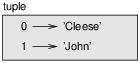
\includegraphics{statediagram12-01}\hfill
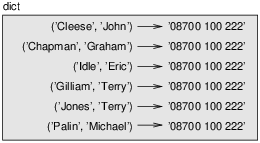
\includegraphics{statediagram12-02}
\end{frame}

\bfr{Sequences: random advice}

\bi
\li Lists, tuples, and strings are often interchangeable.
\li Strings are the most constrained, lists the least.
\li Lists are the only mutable one.
\li Sometimes it's syntactically simpler to use a tuple:

{\lstinline{return a, b, c}}
\li Dictionary keys can't be lists.
\li Passing a tuple to a function instead of a list reduces aliasing.
\li Tuples can't use \lstinline{sort} and \lstinline{reverse}, but
they can use \lstinline{sorted} and \lstinline{reversed}


\ei

\end{frame}

\bfr{Textbook provides a {\tt structshape} module}

\begin{lstlisting}
>>> from structshape import structshape
>>> t = [1, 2, 3]
>>> structshape(t)
'list of 3 int'
>>> t2 = [[1,2], [3,4], [5,6]]
>>> structshape(t2)
'list of 3 list of 2 int'
>>> t3 = [1, 2, 3, 4.0, '5', '6', [7], [8], 9]
>>> structshape(t3)
'list of (3 int, float, 2 str, 2 list of int, int)'
>>> s = 'abc'
>>> lt = list(zip(t, s))
>>> structshape(lt)
'list of 3 tuple of (int, str)'
>>> d = dict(lt) 
>>> structshape(d)
'dict of 3 int->str'
\end{lstlisting}
\end{frame}

\bfr{Vocabulary}
\begin{description}
\li[tuple:]
An immutable sequence of elements.
\li[tuple assignment:]
An assignment with a sequence on the right side and a tuple of variables on the left. The right side is evaluated and then its elements are assigned to the variables on the left.
\li[gather:]
An operation that collects multiple arguments into a tuple.
\li[scatter:]
An operation that makes a sequence behave like multiple arguments.
\end{description}
\end{frame}

\bfr{Vocabulary}
\begin{description}
\li[zip object:]
The result of calling a built-in function zip; an object that iterates through a sequence of tuples.
\li[iterator:]
An object that can iterate through a sequence, but which does not provide list operators and methods.
\li[data structure:]
A collection of related values, often organized in lists, dictionaries, tuples, etc.
\li[shape error:]
An error caused because a value has the wrong shape; that is, the wrong type or size.
\end{description}
\end{frame}


\end{document}
